\subsection{UML Deployment Diagram}
Mediante l’utilizzo di un Deployment Diagram UML è possibile mostrare la rappresentazione hardware e software del sistema. In Figura \ref{fig:uml-deployment-diagram} vengono mostrati i componenti contenuti nei seguenti nodi:


\begin{itemize}
    \item \textbf{Admin}: Interfaccia web utilizzata da un utente admin per creare, gestire e aggiungere membri ai gruppi. Il nodo contiene il componente \textit{AppUserMngt} per la gestione degli utenti.
    
    \item \textbf{User}: Interfaccia web utilizzata dagli utenti per accedere alla piattaforma e gestire i gruppi. Contiene i componenti front-end \textit{AppUserMngt} per la gestione dell'account utente e \textit{GroupMngt} per la gestione dei gruppi.
    
    \item \textbf{Web Server}: Nodo server che espone le API necessarie per la gestione degli utenti e dei gruppi. Contiene i seguenti componenti:
    \begin{itemize}
        \item \textit{AppUserController}: Controller per la gestione delle operazioni relative agli utenti.
        \item \textit{GroupController}: Controller per la gestione delle operazioni sui gruppi.
        \item \textit{AppUser}: Modulo dati per la memorizzazione e gestione delle informazioni utente.
        \item \textit{Group}: Modulo dati per la memorizzazione e gestione delle informazioni sui gruppi.
    \end{itemize}
    
    \item \textbf{Database}: PostgreSQL
\end{itemize}

\begin{figure}[H]
    \centering
    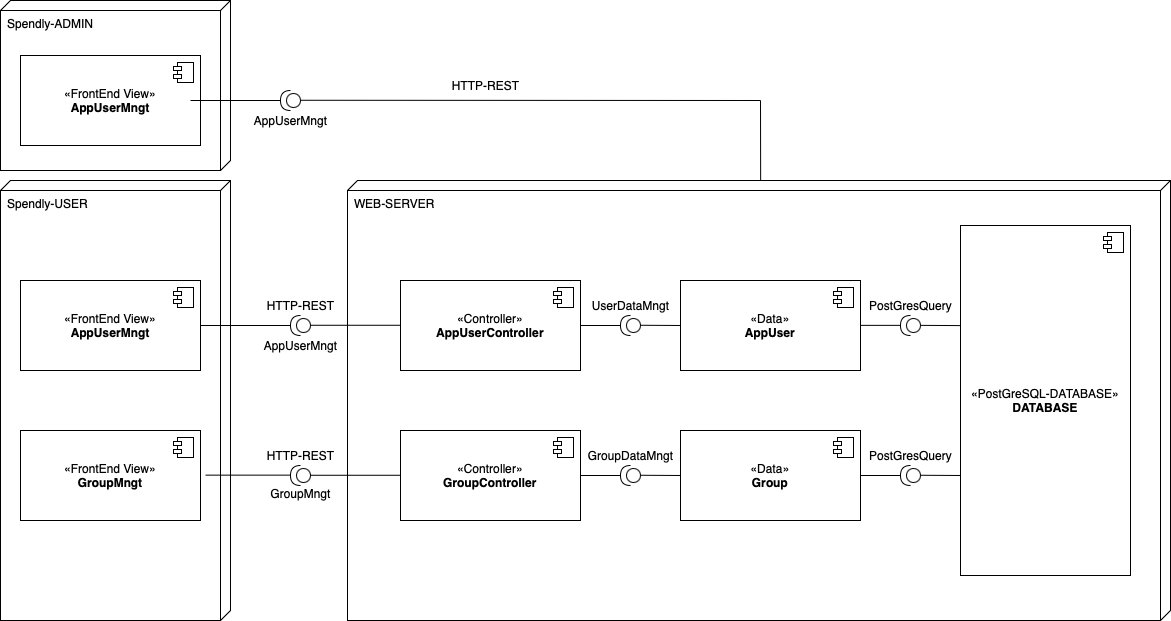
\includegraphics[width=1.1\textwidth, trim=3cm 0cm 1cm 0cm]{images/DeployementDiagramIterazione1.drawio.png}
    \caption{UML Deployment Diagram}
    \label{fig:uml-deployment-diagram}
\end{figure}

